\documentclass[11pt]{article}
\usepackage{latexsym}
\usepackage{amsmath}
\usepackage{amssymb}
\usepackage{amsthm}
\usepackage{epsfig}
\usepackage[tight]{subfigure}
\usepackage{hyperref}

\usepackage{amsmath}

\DeclareMathOperator*{\minimize}{min}
\DeclareMathOperator*{\maximize}{max}

\DeclareMathOperator*{\argmax}{argmax} % thin space, limits underneath in displays
\DeclareMathOperator*{\argmin}{argmin}

\usepackage{algorithm}
 %on linux you may need to run sudo apt-get install texlive-full to install algorithm.sys
\usepackage{algorithmic}

\usepackage{verbatim}

\newcommand{\handout}[5]{
  \noindent
  \begin{center}
  \framebox{
    \vbox{
      \hbox to 5.78in { {#1} \hfill #2 }
      \vspace{4mm}
      \hbox to 5.78in { {\Large \hfill #5  \hfill} }
      \vspace{2mm}
      \hbox to 5.78in { {\em #3 \hfill #4} }
    }
  }
  \end{center}
  \vspace*{4mm}
}

\newcommand{\lecture}[5]{\handout{#1}{#2}{#3}{#4}{#5}}
\newcommand{\collision}[0]{\mathrm{collision}}
\newcommand{\nocollision}[0]{\overline{\collision}}

\newcommand*{\QED}{\hfill\ensuremath{\square}}

\newtheorem{theorem}{Theorem}
\newtheorem{corollary}[theorem]{Corollary}
\newtheorem{lemma}[theorem]{Lemma}
\newtheorem{observation}[theorem]{Observation}
\newtheorem{proposition}[theorem]{Proposition}
\newtheorem{definition}[theorem]{Definition}
\newtheorem{claim}[theorem]{Claim}
\newtheorem{fact}[theorem]{Fact}
\newtheorem{assumption}[theorem]{Assumption}
\newtheorem{note}[theorem]{Note}

% 1-inch margins, from fullpage.sty by H.Partl, Version 2, Dec. 15, 1988.
\topmargin 0pt
\advance \topmargin by -\headheight
\advance \topmargin by -\headsep
\textheight 8.9in
\oddsidemargin 0pt
\evensidemargin \oddsidemargin
\marginparwidth 0.5in
\textwidth 6.5in

\parindent 0in
\parskip 1.5ex
%\renewcommand{\baselinestretch}{1.25}


%%%%% Customize command %%%%%
\newcommand{\btheta}{\boldsymbol{\theta}}
\newcommand{\bz}{\boldsymbol{z}}
\newcommand{\bw}{\boldsymbol{w}}
\newcommand{\bu}{\boldsymbol{u}}
\newcommand{\bv}{\boldsymbol{v}}


\begin{document}

\lecture{Statistical Techniques in Robotics (16-831, S21)}{Lecture \#09
  (Wednesday, March 3)}{Lecturer: Kris Kitani}{Scribes: Chih-Wei Wu, Yu-Jhe Li}{OGD, NormExpGD}

\section{Review}

In the last lecture, we have covered the Online Mirror Decent (OMD), Duality, and the analysis of OMD. We will review some significant points for each of these topics as follows:

\subsection{Online Mirror Descent (OMD)}

Before we directly go into OMD, recall we need to define some notation first and demonstrate how to generalize Follow the Regularized Leader (FTRL) w/ linear loss to OMD. To generalize FTRL linear loss sum, we should have the following notations:
\begin{enumerate}
    \item $\bz^{(1:t)} = \sum_{i=1}^{t} \bz^{(i)}$  (sum of gradients)
    \item $\btheta \triangleq -\bz^{(1:t)}$ (iterating in the dual space)
    \item $\btheta^{(t+1)} = \btheta^{(t)} - \bz^{(t)}$ (parameter of the dual space)
\end{enumerate}

% Then we can derive:
% \begin{align}
%     \bw^{(t+1)} = & \argmax_{\bw} \langle \bw, -\bz^{(1:t)}\rangle -  \psi(\bw) \nonumber \\
%     = & \argmax_{\bw} \langle \bw, \btheta^{(t+1)}\rangle -  \psi(\bw) \nonumber \\
%     = & g(\btheta^{(t+1)}) \nonumber
% \end{align}

We can have the mirror linking function (from dual space $\theta$ to primal space $w$.):
$$\bw = g (\btheta)$$
The algorithm of Online Mirror Decent is presented in the Algorithm~\ref{algo:omd}. 

\begin{algorithm}[H]
\caption{Online Mirror Decent (Convex set $S$, $g: \mathbb{R}^D \rightarrow S$)}
\label{algo:omd}
\begin{algorithmic}[1]
%
\FOR{$t=1,\;\cdots,\;T$}
%
\STATE \textsc{Receive} ($\pmb{f}^{(t)}: S \rightarrow R$) \hfill $\triangleright$ Receive function
%
\STATE $\btheta^{(t+1)} =  \btheta^{(t)} - \eta \bz ^{(t)}$, $\bz \in \partial f^{(t)}(\bw^{(t)})$ \hfill $\triangleright$ Dual parameter update
%
% \STATE \textsc{Receive} ($y^{(t)}\in\{-1, 1\}$) \hfill $\triangleright$ Receive actual answer
%
\STATE $\bw_n^{(t+1)}\leftarrow g\left(\btheta^{(t+1)}\right)$ \hfill $\triangleright$ Mirror projection
%
\ENDFOR
\end{algorithmic}
\end{algorithm}


\subsection{Duality}

% In order to analyze Online Mirror Descent, we need to understand duality which includes Convex Conjugate and Bregman Divergence.

\subsubsection{Convex Conjugate}
Conjugate function is defined as:
\begin{align}
\psi^* (\btheta) = \maximize_{\bw} \left( \langle \btheta, \bw\rangle - \psi (\bw) \right) \nonumber
\end{align}

% 

% Then we can have the geometry of tangent as shown below in the Figure~\ref{fig:tangent}:

% \begin{figure}[H]
% \begin{center}
% 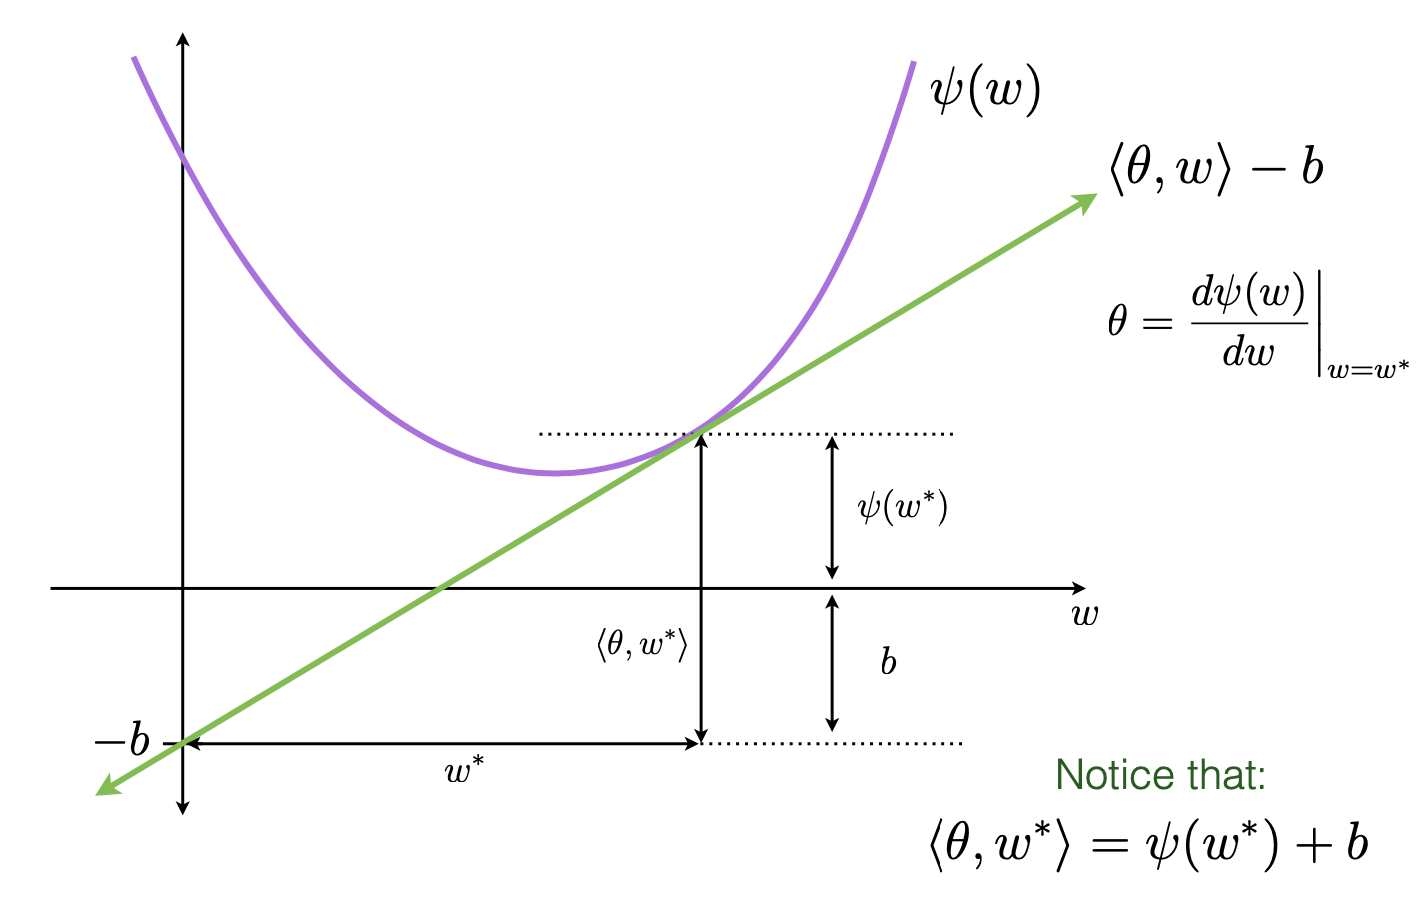
\includegraphics[width=0.7\linewidth]{Img/geometry_tangent.png}
% \end{center}
% \vspace{-10mm}
%  \caption{Geometry of Tangents}
% \label{fig:tangent}
% \end{figure}
% For a corresponding pair $\{ \theta, w^*\}$, we can get:
% $$-b = - \langle \btheta, \bw^* \rangle + \psi (\bw^*).$$
The geometry of the conjugate can be seen as the intercept.

% \begin{figure}[H]
% \begin{center}
% 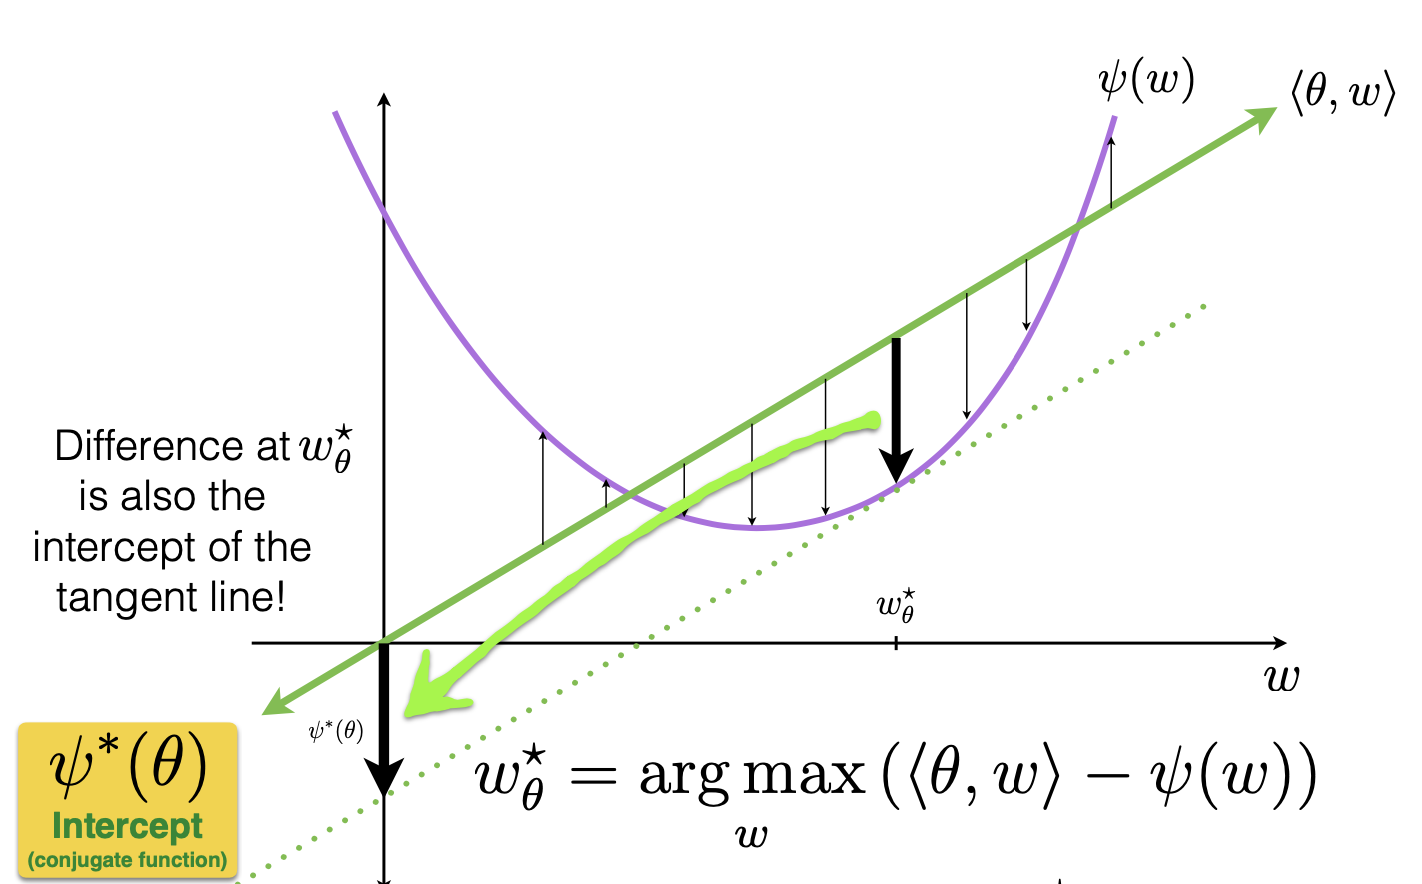
\includegraphics[width=0.7\linewidth]{Img/geometry_conjugate.png}
% \end{center}
% \vspace{-5mm}
%  \caption{Geometry of Conjugate}
% \label{fig:conjugate}
% \end{figure}

\subsubsection{The property of convex conjugate}
Derivative of the convex conjugate is:
\begin{align}
\nabla_{\btheta} \psi^* (\btheta) = & \nabla_{\btheta} \maximize_{\bw} \left( \langle \btheta, \bw \rangle - \psi (\bw)\right) \nonumber
= \nabla_{\btheta} \left( \langle \btheta, \bw^* \rangle - \psi (\bw^*)\right) \nonumber
= \bw^* \nonumber
\end{align}
Slope the convex function is:
$$\nabla_{\bw} \psi (\bw) = \left. \frac{\partial \psi (\bw)}{\partial \bw} \right|_{\bw=\bw^*} = \btheta$$

\subsubsection{Fenchel-Young Inequality}
Since we have the definition: 
\begin{align}
\psi^* (\btheta) = \maximize_{\bw} \left( \langle \btheta, \bw\rangle - \psi (\bw) \right), \nonumber
\end{align}
the Fenchel-Young Inequality can be defined as:
\begin{align}
\psi^* (\btheta) \geq \left( \langle \btheta, \bw\rangle - \psi (\bw) \right) \nonumber
\end{align}

\subsubsection{Bregman Divergence}

Bregman Divergence denotes the ``distance" between two points according to some proximity function $\psi$, which can be defined as:
$$D_{\psi} (\bw||\bu) = \psi(\bw) - \psi(\bu) - \nabla \psi(\bu)^{\top} (\bw-\bu).$$

% Bregman divergence is the approximation error between a linear approximation of some convex function.
% Figure~\ref{fig:breg55}.
% \begin{figure}[H]
% \begin{center}
% 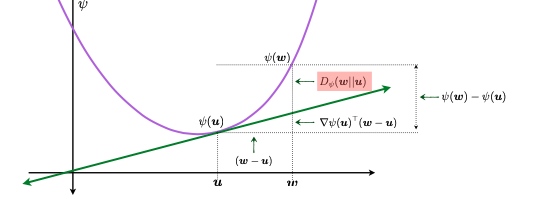
\includegraphics[width=0.7\linewidth]{Img/bredman.png}
% \end{center}
% \vspace{-5mm}
%  \caption{Bredman divergence.}
% \label{fig:breg55}
% \end{figure}

\subsection{OMD Analysis}

Now that we have the mathematical tools introduced in the previous section, we could derive the regret bound for Online Mirror Descent algorithm. The regret bound for Online Mirror Descent algorithm is:
%
\begin{equation*}
\begin{split}
R(\boldsymbol{u}) &= \sum_{t=1}^{T} \boldsymbol{w}^{(t)} \cdot \boldsymbol{z}^{(t)} - \boldsymbol{u} \cdot \boldsymbol{z}^{(t)} \\
& \leq \psi(\boldsymbol{u}) - \psi(\boldsymbol{w}^{(1)}) + \sum_{t=1}^{T} D_{\psi^*} (-\boldsymbol{z}^{(1:t)} || -\boldsymbol{z}^{(1:t-1)})
\end{split}
\end{equation*}
%
The first two terms $\psi(\boldsymbol{u}) - \psi(\boldsymbol{w}^{(1)})$ come from the \textbf{regularization function}, and the last term $\sum_{t=1}^{T} D_{\psi^*} (-\boldsymbol{z}^{(1:t)} || -\boldsymbol{z}^{(1:t-1)})$ comes from \textbf{Bregman Divergence under the convex conjugate of the regularization function}.


%%% PROOF %%%%%


% To proof the regret bound, we start from the loss function of an arbitrary:
% \begin{equation*}
% \begin{split}
% \psi (\boldsymbol{u}) + \sum_{t=1}^T \boldsymbol{u} \cdot \boldsymbol{z}^{(t)} \\
% = \psi (\boldsymbol{u}) - \boldsymbol{u} \cdot \btheta^{(T+1)}
% \end{split}
% \end{equation*}

% By applying Fenchel-Young Inequality $\psi^* (\boldsymbol{\theta}) \geq (\langle \boldsymbol{w}, \boldsymbol{\theta} \rangle - \psi (\boldsymbol{w}))$ to RHS:
% \begin{equation*}
% \begin{split}
% \psi (\boldsymbol{u}) - \boldsymbol{u} \cdot \btheta^{(T+1)} \geq -\psi^*(\btheta^{(T+1)})
% \end{split}
% \end{equation*}

% Next, we expand the RHS with telescoping~\cite{telescoping}. It is conducted as follows:
% \begin{equation*}
% \begin{split}
% -\psi^*(\btheta^{(T+1)}) &= 
% -\psi^*(\btheta^{(T+1)})
% -\psi^*(\btheta^{(T)})
% +\psi^*(\btheta^{(T)})
% -\cdots
% -\psi^*(\btheta^{(1)})
% +\psi^*(\btheta^{(1)}) \\
% &= -\psi^*(\btheta^{(1)}) 
% -\sum^{T}_{t=1} \Big( \psi^*(\btheta^{(t+1)}) - \psi^*(\btheta^{(t)}) \Big)
% \end{split}
% \end{equation*}

% The first term can be written as $\psi(\boldsymbol{w}^{(1)})$. And the second summation term can written as $-\sum_{t=1}^{T} \Big( \nabla \psi^*(\btheta^{(t)}) \cdot (\btheta^{(t+1)} - \btheta^{(t)}) + D_{\psi^*} (\btheta^{(t+1)} || \btheta^{(t)}) \Big)$ by plugging in the definition of Bregman Divergence. The whole could be written as:
% \begin{equation*}
% \begin{split}
% -\psi^*(\btheta^{(T+1)}) &=
% -\psi(\boldsymbol{w}^{(1)}) 
% -\sum_{t=1}^{T} \Big( \nabla \psi^*(\btheta^{(t)}) \cdot (\btheta^{(t+1)} - \btheta^{(t)}) + D_{\psi^*} (\btheta^{(t+1)} || \btheta^{(t)}) \Big)
% \end{split}
% \end{equation*}

% By definition of the dual parameter $\btheta^{(t+1)} \triangleq -\bz^{(1:t-1)}$, we could have:
% \begin{equation*}
% \begin{split}
% -\psi^*(-\bz^{(1:T)}) &=
% -\psi(\boldsymbol{w}^{(1)}) 
% -\sum_{t=1}^{T} \Big( \nabla \psi^*(-\bz^{(1:t-1)}) \cdot (-\bz^{(1:t)} + \bz^{(1:t-1)}) + D_{\psi^*} (-\bz^{(1:t)} || -\bz^{(1:t-1)}) \Big) \\
% &= \psi(\boldsymbol{w}^{(1)}) 
% -\sum_{t=1}^{T} \Big( \langle \bw^{(t)}, -\bz^{(t)} \rangle
% + D_{\psi^*} (-\bz^{(1:t)} || -\bz^{(1:t-1)}) \Big) \\
% &= \psi(\boldsymbol{w}^{(1)}) 
% +\sum_{t=1}^{T} \Big( \langle \bw^{(t)}, \bz^{(t)} \rangle
% - D_{\psi^*} (-\bz^{(1:t)} || -\bz^{(1:t-1)}) \Big) \\
% \psi^*(-\bz^{(1:T)}) &= -\psi(\boldsymbol{w}^{(1)}) 
% -\sum_{t=1}^{T} \Big( \langle \bw^{(t)}, \bz^{(t)} \rangle
% - D_{\psi^*} (-\bz^{(1:t)} || -\bz^{(1:t-1)}) \Big)
% \end{split}
% \end{equation*}

% Now back to the Fenchel-Young Inequality we infer at the start of this proof, $\psi (\boldsymbol{u}) - \boldsymbol{u} \cdot \btheta^{(T+1)} \geq -\psi^*(\btheta^{(T+1)})$ could be written as:
% \begin{equation*}
% \begin{split}
% \langle \bu,-\bz^{(1:T)} \rangle
% -\psi(\bu)
% &\leq \psi^*(-\bz^{(1:T)}) \\
% \langle \bu,-\bz^{(1:T)} \rangle
% -\psi(\bu)
% &\leq -\psi(\boldsymbol{w}^{(1)}) 
% -\sum_{t=1}^{T} \Big( \langle \bw^{(t)}, \bz^{(t)} \rangle
% -D_{\psi^*} (-\bz^{(1:t)} || -\bz^{(1:t-1)}) \Big) \\
% \langle \bu,-\bz^{(1:T)} \rangle
% -\psi(\bu)
% &\leq -\psi(\boldsymbol{w}^{(1)}) 
% -\sum_{t=1}^{T} \langle \bw^{(t)}, \bz^{(t)} \rangle
% +\sum_{t=1}^{T} D_{\psi^*} (-\bz^{(1:t)} || -\bz^{(1:t-1)}) \\
% \sum_{t=1}^{T} \langle \bw^{(t)}, \bz^{(t)} \rangle
% -\langle \bu,\bz^{(1:T)} \rangle
% &\leq \psi(\bu)
% -\psi(\boldsymbol{w}^{(1)}) 
% +\sum_{t=1}^{T} D_{\psi^*} (-\bz^{(1:t)} || -\bz^{(1:t-1)})
% \end{split}
% \end{equation*}

% The LHS is actually the definition of regret. So the regret bound of Online Mirror Descent is proved as:
% \begin{equation*}
% \begin{split}
% R(\bu)=\sum_{t=1}^{T} \langle \bw^{(t)}, \bz^{(t)} \rangle
% -\langle \bu,\bz^{(1:T)} \rangle
% &\leq \psi(\bu)
% -\psi(\boldsymbol{w}^{(1)}) 
% +\sum_{t=1}^{T} D_{\psi^*} (-\bz^{(1:t)} || -\bz^{(1:t-1)})
% \end{split}
% \end{equation*}



\section{Summary}

\subsection{Online Gradient Decent}
\subsubsection{Gradient Descent}

Gradient descent is pretty much a standard approach for minimizing differentiable convex functions. In this lecture, we provide 3 perspectives to understand how gradient descent works.

\textbf{Perspective 1: Geometric.}
The geometric intuition of gradient descent is illustrated in Figure~\ref{fig:GD_geometric}. Given a convex and differentiable function $f:\mathbb{R}^N \rightarrow \mathbb{R}$, its gradient $\nabla f(\bw)$ at $\bw$ could be calculated with $\nabla f(\bw) = \{ \frac{\partial f(\bw)}{w_1}, \cdots, \frac{\partial f(\bw)}{w_N} \}$.
%
% \begin{equation*}
% \begin{split}
% \nabla f(\bw) = \Bigg\{ \frac{\partial f(\bw)}{w_1}, \cdots, \frac{\partial f(\bw)}{w_N} \Bigg\}
% \end{split}
% \end{equation*}
%
To find the minima of $f$, by moving step by step in the opposite direction of the gradient, we would eventually arrive at the minima of $f$. The complete algorithm of gradient descent is presented in Algorithm~\ref{algo:gd}.

\begin{figure}[t]
    \centering
    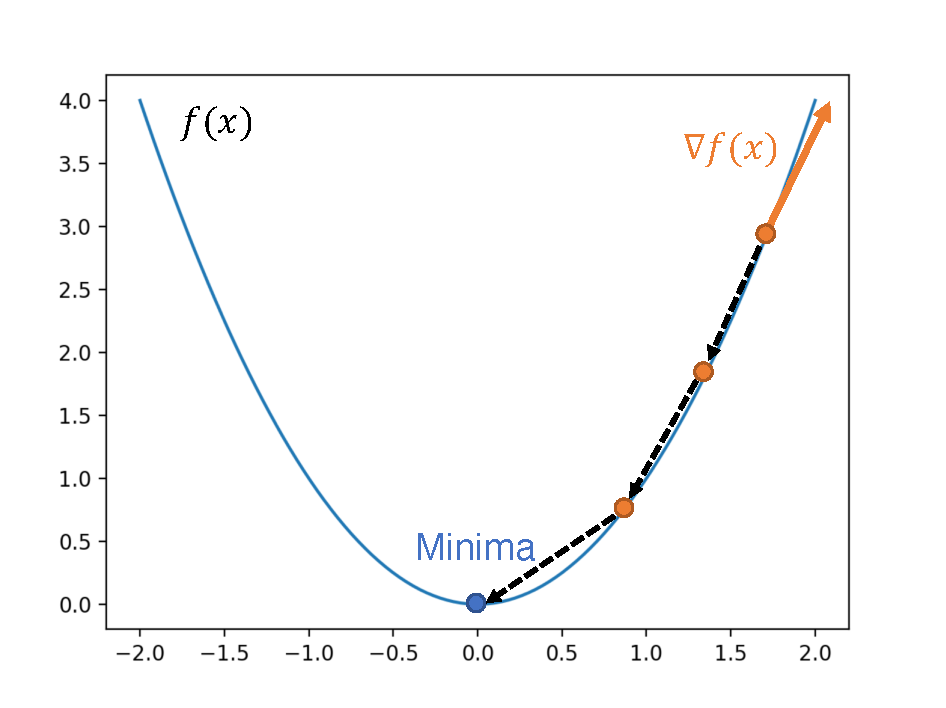
\includegraphics[width=0.4\textwidth]{Img/gradient_descent.pdf}
    \caption{Geometric meaning of gradient descent.
    %To find the minima of $f$, we should move in the opposite direction of the gradient step by step.
    }
    \label{fig:GD_geometric}
\end{figure}

\begin{algorithm}[H]
\caption{Gradient Decent ($f$)}
\label{algo:gd}
\begin{algorithmic}[1]
\STATE $\bw^{(0)} \leftarrow \boldsymbol{0}$
\FOR{$t=1,\;\cdots,\;T$}
\STATE \textsc{Compute}($\nabla f(\bw^{(t-1)})$)
\STATE $\bw^{(t)} = \bw^{(t-1)} - \eta \nabla f(\bw^{(t-1)})$
\ENDFOR
\end{algorithmic}
\end{algorithm}

\textbf{Perspective 2: Linear approximation with regularization.}
Mathematically, for a convex function $f:\mathbb{R}^N \rightarrow \mathbb{R}$, we could lower bound its value at $\bw$ with Taylor series approximation at $\bu$:
%This concept is illustrated in Figure~\ref{fig:GD_lin_apprx}.
%Formally:
%
\begin{equation*}
\begin{split}
f(\bu) \leq f(\bw) + \langle \bu-\bw, \nabla f(\bw) \rangle
\end{split}
\end{equation*}
%
The RHS serves as an approximation for $f(\bw)$, however, with a constraint. If we minimize the RHS, it would diverge to negative infinity instead of converging to the local minima of $f$. The reason is that the approximation is only accurate for values close to $\bw$.
To factor in this constraint, we should constrain the distance between $\bw$ and $\bu$ with squared L2 norm, i.e. $\min_w \| \bu - \bw \|_2^2$. Hence, to find the minima of function $f$, we should optimize the following objective function: 
%
\begin{equation*}
\begin{split}
\min_{\bw} \frac{1}{2} \| \bu - \bw \|_2^2 
+ \eta\Big(f(\bw) + \langle \bu-\bw, \nabla f(\bw) \rangle \Big)
\end{split}
\end{equation*}
%
And to find the $w$ that minimizes the function $f$: (Note that we substitute $\bu$ with $\bw$, substitute $\bw$ with $\bw^{(t)}$)
%
\begin{equation*}
\begin{split}
\bw^{(t+1)} = 
\underset{\bw}{\arg\min} \frac{1}{2} \| \bw - \bw^{(t)} \|_2^2 
+ \eta\Big(f(\bw^{(t)}) + \langle \bw-\bw^{(t)}, \nabla f(\bw^{(t)}) \rangle \Big)
\end{split}
\end{equation*}
%
The above equation is similar to the update step in Online Mirror Descent, where it optimizes a linear loss function with quadratic regularization.

% \begin{figure}[H]
%     \centering
%     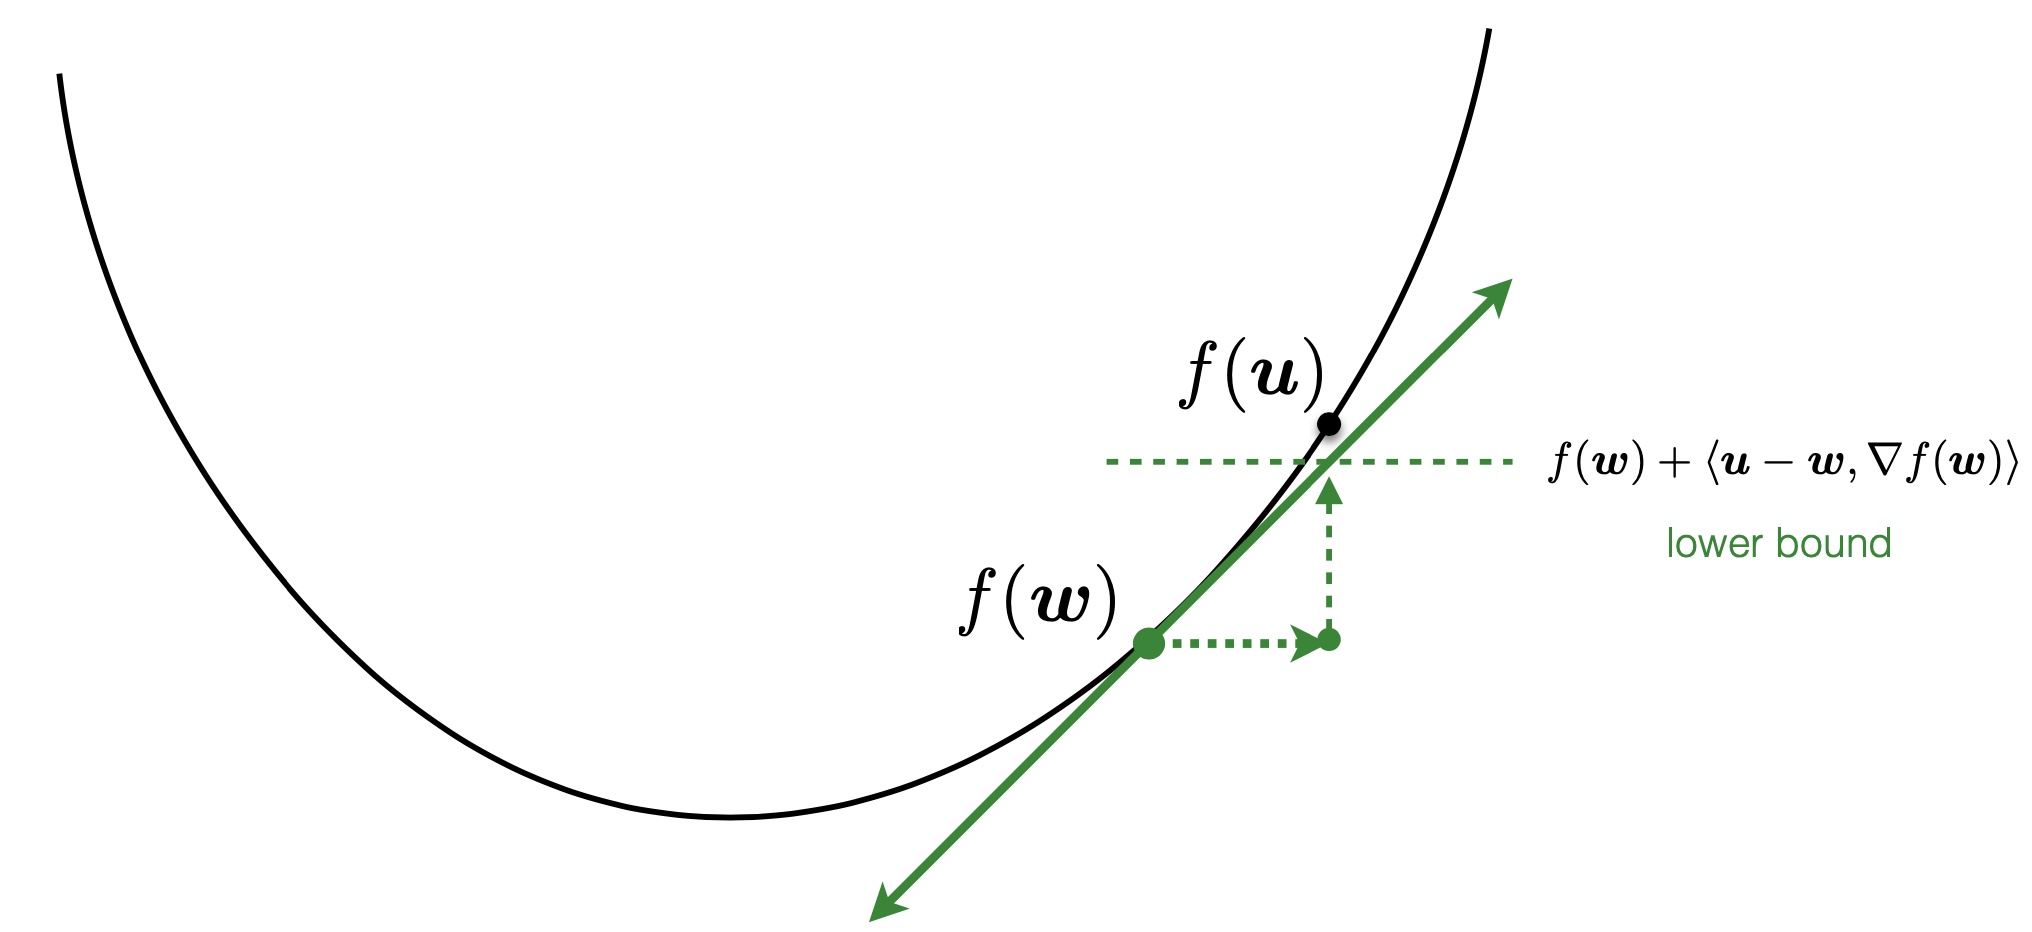
\includegraphics[width=0.5\textwidth]{Img/GD_lin_apprx.png}
%     \caption{Lower bounding $f(\bu)$ with Taylor series at $\bw$.}
%     \label{fig:GD_lin_apprx}
% \end{figure}

\textbf{Perspective 3: Isometric quadratic approximation.}
According Tayler expansion, we know that we could approximate a function $f$ at $\bu$ with a nearby location $\bw$ by the following:
%
\begin{equation*}
\begin{split}
f(\bu) \approx f(\bw) + (\bu-\bw)^T \nabla f(\bw) + \frac{1}{2} (\bu-\bw)^T \nabla^2 f(\bw) (\bu-\bw)
\end{split}
\end{equation*}
%
For a function that is L-smooth, we could derive its upper bound function by the isometric quadratic approximation:
%And according to isometric quadratic approximation, the upper bound function of the above approximation could also approximate the function $f$:
\begin{equation*}
\begin{split}
f(\bu) \approx f(\bw) + (\bu-\bw)^T \nabla f(\bw) + \frac{1}{2\eta} (\bu-\bw)^T \boldsymbol{I} (\bu-\bw),
\end{split}
\end{equation*}
where $\eta$ is a tunable variance parameter. For the proof that the above approximation is an upper bound of a L-smooth function, please refer to Appendix~\ref{sec:l_smooth}.
%An illustration of the relation between these approximation functions and the original function $f$ is presented in Figure~\ref{fig:GD_iso_quad}. 
%
% \begin{figure}[H]
%     \centering
%     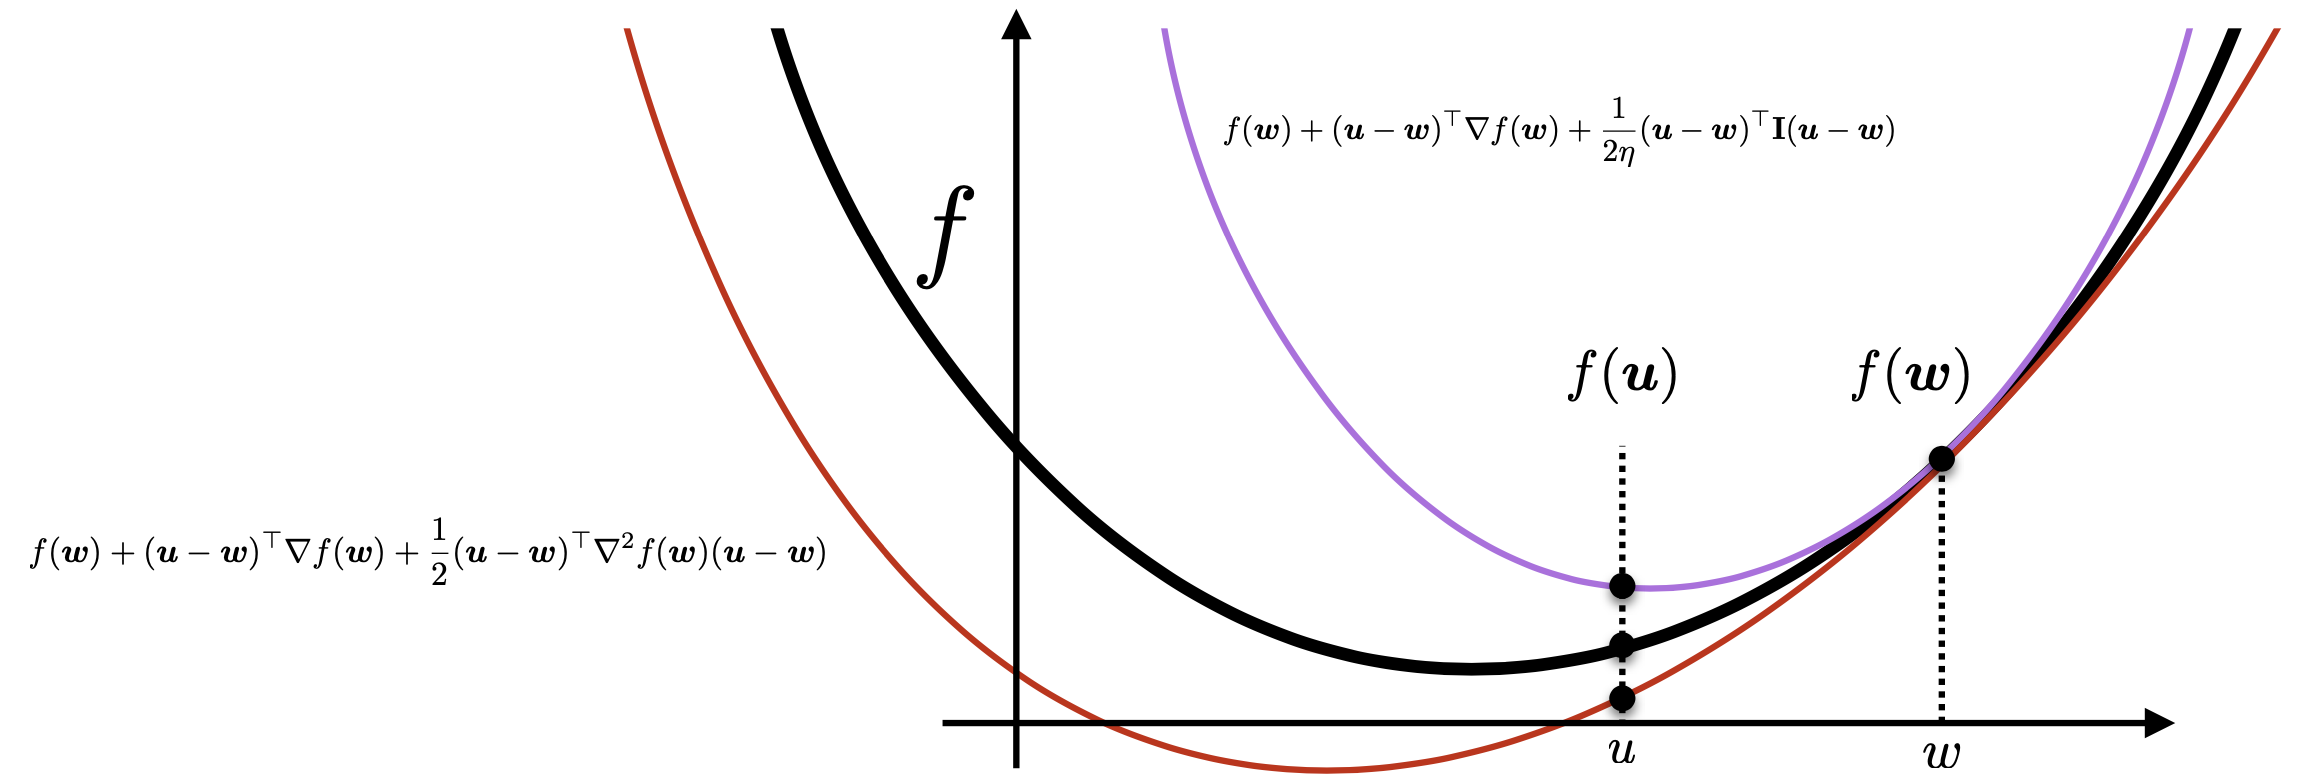
\includegraphics[width=0.8\textwidth]{Img/GD_iso_quad.png}
%     \caption{The Taylor series approximation and isometric quadratic approximation of $f$.}
%     \label{fig:GD_iso_quad}
% \end{figure}
%
To obtain the minima of $f$, one could optimize for the second approximated function:
\begin{equation*}
\begin{split}
%&\underset{\bw}{\arg\min} f(\bw) + (\bu-\bw)^T \nabla f(\bw) + \frac{1}{2\eta} (\bu-\bw)^T \boldsymbol{I} (\bu-\bw) \\
\underset{\bw}{\arg\min} \frac{1}{2} \|\bu-\bw\|^2 +
\eta \Big( f(\bw) + (\bu-\bw)^T \nabla f(\bw) \Big)
\end{split}
\end{equation*}

By substituting $\bu$ with $\bw$, substituting $\bw$ with $\bw^{(t)}$, the formulation is same with \textbf{perspective 2}:
\begin{equation*}
\begin{split}
\bw^{(t+1)} = 
\underset{\bw}{\arg\min} \frac{1}{2} \| \bw - \bw^{(t)} \|_2^2 
+ \eta\Big(f(\bw^{(t)}) + \langle \bw-\bw^{(t)}, \nabla f(\bw^{(t)}) \rangle \Big)
\end{split}
\end{equation*}

To obtain the minima, we use the simple method of deriving its gradient and find the solution of the gradient:
%
\begin{equation*}
\begin{split}
%\frac{\partial}{\partial\bw}\Bigg\{ 
%\frac{1}{2} \| \bw - \bw^{(t)} \|_2^2 
%+ \eta\Big(f(\bw^{(t)}) + \langle \bw-\bw^{(t)}, \nabla f(\bw^{(t)}) \rangle \Big)
%\Bigg\} &= 0 \\
%\frac{1}{2}\Big( \bw+0-2\bw^{(t)} \Big)
%\eta \Big( 0 + \nabla f(\bw^{(t)}) - 0 \Big) &= 0 \\
%\bw - \bw^{(t)} + \eta \nabla f(\bw^{(t)}) &= 0 \\
\bw = \bw^{(t)} - \eta \nabla f(\bw^{(t)})
\end{split}
\end{equation*}
%
This displays resemblance to the update rule of the Weighted Majority Algorithm, 
Online Perceptron Algorithm, and the Follow The Regularized Leader Algorithm. In short, the final equation is the solution to the gradient descent on the function $f$ from a \textbf{quadratic approximation} of the loss function $f$.

\subsubsection{Stochastic Gradient Descent}
Although gradient descent is guaranteed to reach the local minimum mathematically, its computation speed is not desirable in practice. The problem is that computing gradient of the function $\nabla f$ over all training example is expensive sometimes. An alternative is to perform the \textbf{Stochastic Gradient Descent}, where instead of updating parameter after computing gradient of all examples, it updates the parameter after computing each example's gradient. An overview of the stochastic gradient descent is demonstrated in Algorithm~\ref{algo:sgd}.
%
%The steps of Stochastic Gradient Descent is as follows. First, we initialize the weight $\bw$ to 0 and set the learning parameter $\eta$. Then for each iteration, we extract a sample or a mini-batch of samples from the data distribution. We then calculate their gradients and update the weight. 
In comparison to the vanilla gradient descent, computing the gradient of single sample or part of the full data is much faster. Although the direction of each iteration would not always point at the descending direction, the expected value of the direction would equal the gradient direction. Consequently, stochastic gradient descent has similar convergence bound as gradient descent.

\begin{algorithm}[H]
\caption{Stochastic Gradient Decent ($f$)}
\label{algo:sgd}
\begin{algorithmic}[1]
\STATE $\bw^{(1)} \leftarrow \boldsymbol{0}$
\STATE $\eta > 0$
\FOR{$t=1,\;\cdots,\;T$}
\STATE $z\sim\mathcal{D}$ \hfill $\triangleright$ Sample single sample from data distribution
\STATE $\bv^{(t)} = \nabla f_z(\bw^{(t-1)})$ \hfill $\triangleright$ Fast to compute
\STATE $\bw^{(t)} = \bw^{(t-1)} - \eta\bv^{(t)}$
\ENDFOR
\end{algorithmic}
\end{algorithm}

\subsubsection{Online (Projected Sub-) Gradient Descent as OMD}


\begin{figure}[t]
    \centering
    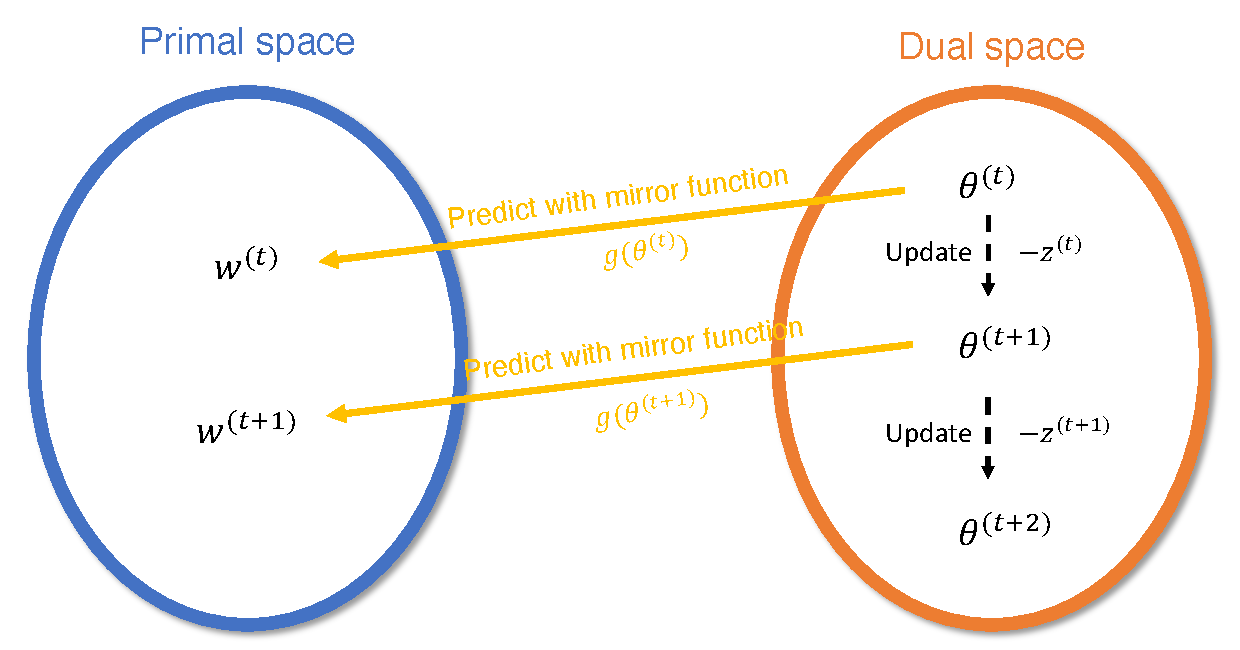
\includegraphics[width=0.7\textwidth]{Img/dual_space.pdf}
    \caption{Dual space of the Online Mirror Descent.}
    \label{fig:dual_space}
\end{figure}

In this subsection, we are going to show that Online Gradient Descent is a special case of Online Mirror Descent (OMD). Recall that the Online Mirror Descent updates its primal parameter with the dual parameter by a mirror function $g(\btheta)$, as shown in Figure~\ref{fig:dual_space}. The mirror function, or aliased with weight prediction rule, is written as: 
%
\begin{equation*}
\begin{split}
\bw^{(t+1)} = \underset{\bw}{\arg\min} \langle \bw,-\btheta^{(t+1)} \rangle
+\psi(\bw)
\end{split}
\end{equation*}
%
Online Gradient Descent is just a special case of Online Mirror Descent, by defining 
this \textbf{quadratic regularization function}: $\phi(\bw) = \frac{1}{2\eta}\|\bw\|^2_2$, and defining a \textbf{linear loss function}: $f(\bw)=\langle \bw, \btheta \rangle$. Namely, the weight prediction rule for Online Gradient Descent is written as:
%
\begin{equation*}
\begin{split}
\bw^{(t+1)} = \underset{\bw}{\arg\min} \langle \bw,-\btheta^{(t+1)} \rangle
+\frac{1}{2\eta}\|\bw\|^2_2
\end{split}
\end{equation*}
%
Furthermore, we could derive the minimization function by finding the solution of its gradient:
\begin{equation*}
\begin{split}
%\bw^{(t+1)} 
%&= \underset{\bw}{\arg\min} \langle \bw,-\btheta^{(t+1)} \rangle
%+\frac{1}{2\eta}\|\bw\|^2_2 \\
%&= \underset{\bw}{\arg\min} \langle \bw,-\btheta^{(t+1)} \rangle
%+\frac{1}{2\eta}\sum_n w^2_n \\
\mathcal{L} &= \langle \bw,-\btheta^{(t+1)} \rangle
+\frac{1}{2\eta}\sum_n w^2_n \\
\frac{\partial\mathcal{L}}{\partial w_n}
&= \theta_n + \frac{1}{2\eta} 2w_n = 0 \\
&\Rightarrow w_n = -\eta \theta_n
\end{split}
\end{equation*}

The last equation actually projects the parameter in the dual space back into the parameter in the primal space.
Therefore, we conclude the mirror function for Online Gradient Descent is:
%
\begin{equation*}
\begin{split}
g(\btheta) = -\eta \btheta
\end{split}
\end{equation*}
%
There is actually 2 variants of the Online Gradient Descent mirror function. The first one uses the above weight prediction rule under the assumption that the sub-gradient of the function is constraint within certain range. This is called the Online Sub-Gradient Descent, as depicted in Algorithm~\ref{algo:osgd}. The second one adds a convex set projection function to the weight prediction rule: $g(\btheta) = \prod_{\theta \rightarrow S} (-\eta \btheta)$. This is called the Online Projected Sub-Gradient Descent, as displayed in Algorithm~\ref{algo:opsgd}. Both of them falls into the family of Online Gradient Descent, which we that it is a special case of Online Mirror Descent with linear loss and quadratic regularizer.

\begin{algorithm}[H]
\caption{Online Sub-Gradient Decent ($\eta$)}
\label{algo:osgd}
\begin{algorithmic}[1]
\FOR{$t=1,\;\cdots,\;T$}
\STATE $\btheta^{(t+1)} =  \btheta^{(t)} - \eta \bz ^{(t)}$, $\bz \in \partial f^{(t)}(\bw^{(t)})$ \hfill $\triangleright$ Dual parameter update
\STATE $\bw_n^{(t+1)} = -\eta \btheta$ \hfill $\triangleright$ Mirror projection
\ENDFOR
\end{algorithmic}
\end{algorithm}


\begin{algorithm}[H]
\caption{Online Projected Sub-Gradient Decent ($\eta$)}
\label{algo:opsgd}
\begin{algorithmic}[1]
\FOR{$t=1,\;\cdots,\;T$}
\STATE $\btheta^{(t+1)} =  \btheta^{(t)} - \eta \bz ^{(t)}$, $\bz \in \partial f^{(t)}(\bw^{(t)})$ \hfill $\triangleright$ Dual parameter update
\STATE $\bw_n^{(t+1)} = \prod_{\theta \rightarrow S}-\eta \btheta$ \hfill $\triangleright$ Mirror projection
\ENDFOR
\end{algorithmic}
\end{algorithm}

\subsubsection{Online Gradient Descent Analysis}

Now we would like to derive a regret bound as:
\begin{equation*}
\begin{split}
R_{OGD} \leq DG\sqrt{T}
\end{split}
\end{equation*}
where $D=\max\|\bu\|_2, \bu \in S$ (assumption on the magnitude of the primal parameter) and $G=\max \| \bz \|_2, \bz \in \partial f(\bw)$ (assumption on the magnitude of sub-gradient).
%
% \begin{figure}[H]
%     \centering
%     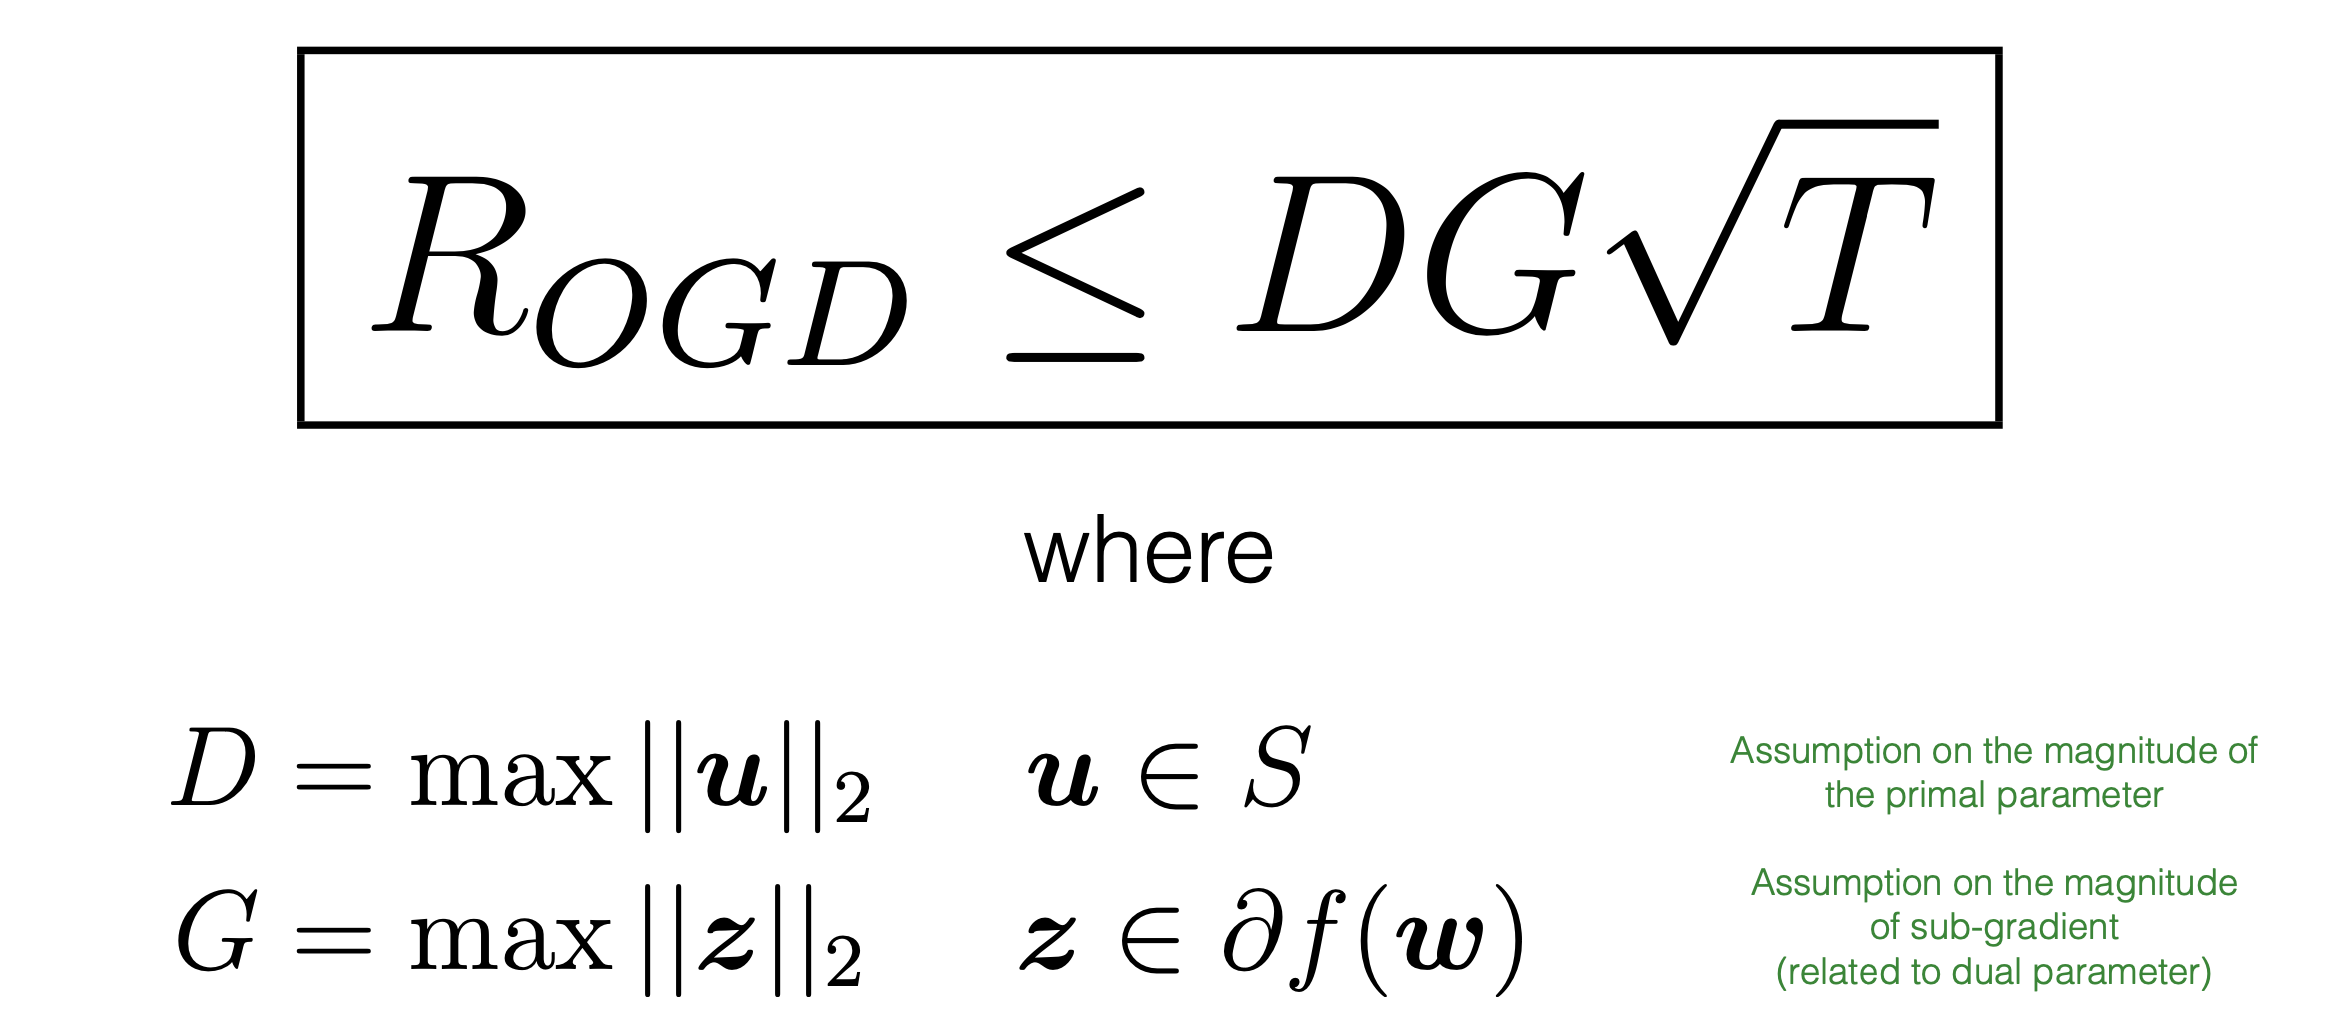
\includegraphics[width=0.7\linewidth]{Img/OGD_regret.png}
%     \label{fig:OGD_regret_}
% \end{figure}
%
Recall the general regret bound as:
%
\begin{equation*}
\begin{split}
R(\bu)=\sum_{t=1}^{T} \langle \bw^{(t)}, \bz^{(t)} \rangle
-\langle \bu,\bz^{(1:T)} \rangle
&\leq \psi(\bu)
-\psi(\boldsymbol{w}^{(1)}) 
+\sum_{t=1}^{T} D_{\psi^*} (-\bz^{(1:t)} || -\bz^{(1:t-1)})
\end{split}
\end{equation*}
%
We can start from the regret bound of OMD to derive the regret bound of OGD:
\begin{equation*}
\begin{split}
R(\bu) \leq
& \psi(\bu)
 -  \psi(\bw^{(1)}) 
 +\sum_{t=1}^{T} D_{\psi^*} (\btheta^{(t+1)} || \btheta^{(t)})\\
= & \psi(\bu)
-  \psi(\bw^{(1)}) 
+ \sum_{t=1}^{T} \psi^*(\btheta^{(t-1)}) - \psi^*(\btheta^{(t)}) - \nabla \psi^*(\btheta^{(t-1)})(\btheta^{(t)}) (\btheta^{(t+1)} - \btheta^{(t)})\\
% = & \frac{1}{2\eta} \|\bu\|_2^2-\frac{1}{2\eta} \|\bw\|_2^2+\sum_{t=1}^T \frac{1}{2\eta} \|\btheta^{(t+1)}\|_2^2 - \|\btheta^{(t)}\|_2^2 - \nabla \frac{1}{2\eta} \|\btheta^{(t)}\|_2^2 (\btheta^{(t+1)}-\btheta^{(t)})\\
= & \frac{1}{2\eta} \|\bu\|_2^2-\frac{1}{2\eta} \|\bw\|_2^2+\sum_{t=1}^T \frac{1}{2\eta} \|\btheta^{(t+1)}\|_2^2 - \|\btheta^{(t)}\|_2^2 - \frac{1}{\eta} \btheta^{(t)} (\btheta^{(t+1)}-\btheta^{(t)})\\
= & \frac{1}{2\eta} \|\bu\|_2^2-\frac{1}{2\eta} \|\bw\|_2^2+\sum_{t=1}^T \frac{1}{2\eta} \|\btheta^{(t+1)} - \btheta^{(t)}\|_2^2\\
= & \frac{1}{2\eta} \|\bu\|_2^2-\frac{1}{2\eta} \|\bw\|_2^2+\sum_{t=1}^T \frac{1}{2\eta} \|(-\bz^{(1:t)}) - (-\bz^{(1:t-1)})\|_2^2\\
% = & \frac{1}{2\eta} \|\bu\|_2^2-\frac{1}{2\eta} \|\bw\|_2^2+\sum_{t=1}^T \frac{1}{2\eta} \|-\bz^{(t)}\|_2^2\\
%
\leq & \frac{1}{2 \eta}||\bu||_2^2 + \sum_{t=1}^T \frac{1}{2 \eta} ||\bz^{(t)}||_2^2 
\end{split}
\end{equation*}
% \begin{align}
%     R(u) \leq & no\\
% \end{align}
Recall:
\begin{align}
    D = &\max ||\bu||_2 \quad \bu\in S \nonumber\\
    G = &\max ||\bz||_2 \quad \bz\in \partial f(\bw) \nonumber
\end{align}
%
So we can derive:
\begin{align}
    % R_{ODG} (\bu) \leq & \frac{1}{2 \eta}||\bu||_2^2 + \sum_{t=1}^T \frac{1}{2 \eta} ||\bz^{(t)}||_2^2  \nonumber\\
    R_{ODG} \leq & \frac{D^2}{2 \eta} + \frac{\eta}{2} T^2 G \nonumber
\end{align}
%
To find the optimal $\eta$, we take the derivative:
\begin{align}
    \frac{d}{d \eta} \left\{ \frac{1}{\eta} D^2 + \frac{\eta}{2} G^2T \right\} = & 0  \rightarrow \eta = \frac{D}{G \sqrt{T}} \nonumber
    % \frac{-D^2}{2 \eta^2} + \frac{G^2 T}{2}= & 0 \nonumber \\
    % \frac{-D^2}{2} + \frac{ \eta^2 G^2 T}{2}= & 0 \nonumber \\
    % \eta^2 = & \frac{D^2}{G^2 T} \nonumber \\
\end{align}
%
Then we can subscribe back to the regret:
\begin{align}
    R_{ODG} (\bu) \leq & \frac{D^2}{2 \eta} + \frac{\eta}{2} T^2 G \nonumber \\
    = & DG \sqrt{T} \nonumber
\end{align}
%
\subsection{Online Normalized Exponentiated
Gradient Descent}

Recall the Online Gradient Decent in the Algorithm~\ref{algo:omd}, we can actually have the Norm-Exponentiated-Gradient summarized in the Algorithm~\ref{algo:onegd}. We will show how we can derive the Normalized Exponentiated Gradient from Algorithm~\ref{algo:omd} to Algorithm~\ref{algo:onegd} in some steps below.
%
% \begin{algorithm}[H]
% \caption{Online Mirror Decent (Convex set $S$, $g: \mathbb{R}^D \rightarrow S$)}
% \label{algo:omd2}
% \begin{algorithmic}[1]
% \FOR{$t=1,\;\cdots,\;T$}
% %
% \STATE \textsc{Receive} ($\pmb{f}^{(t)}: S \rightarrow R$) \hfill $\triangleright$ Receive function
% %
% \STATE $\btheta^{(t+1)} =  \btheta^{(t)} - \eta z ^{(t)}$, $\bz \in \partial f^{(t)}(\bw^{(t)})$ \hfill $\triangleright$ Dual parameter update
% %
% \STATE $\bw_n^{(t+1)} =  g\left(\btheta^{(t+1)}\right)$ \hfill $\triangleright$ Mirror projection
% %
% \ENDFOR
% \end{algorithmic}
% \end{algorithm}
%
%
\begin{algorithm}[H]
\caption{Norm-Exponentiated-Gradient ($\eta$)}
\label{algo:onegd}
\begin{algorithmic}[1]
\FOR{$t=1,\;\cdots,\;T$}
%
\STATE $\bz \in \partial f^{(t)}(\bw^{(t)})$ 
%
\STATE $\bw^{(t+1)} \propto \bw^{(t)} \exp{(\eta \bz^{(t)})}$ 
%
\ENDFOR
\end{algorithmic}
\end{algorithm}
%
In the first place, we will define the regularization function $\psi (w)$ as:
\begin{align}\label{eq:reg}
    \psi (\bw) = \sum_{k=1}^{K} \bw_k \log \bw_k \quad \bw\in \mathbb{S}^K.
\end{align}
%
You may see equation~\ref{eq:reg} as negative entropy and K-simplex constraint. Then when we define the loss as:
$$f(\bw) = \langle \bw, \btheta\rangle,$$
the prediction rule will become:
\begin{align}\label{eq:reg2}
    \bw^{(t+1)} = & \argmin_{\bw} \langle \bw, -\btheta^{(t+1)} \rangle + \psi (\bw)\nonumber \\
    = & \argmin_{\bw \in \mathbb{S}^K} \langle \bw, -\btheta^{(t+1)} \rangle + \sum_{k=1}^{K} \bw_k \log \bw_k
\end{align}
Now we can then add simplex constraint to the objective in the equation~\ref{eq:reg2} as:
\begin{align}
    \bw^{(t+1)} = \argmin_{\bw \in \mathbb{S}^K} \langle \bw, -\btheta^{(t+1)} \rangle + \sum_{k=1}^{K} \bw_k \log \bw_k + \lambda \left( 1- \sum_k \bw_k\right)
\end{align}
The Lagrangian can be derived from the equation as:
$$ \mathcal{L} = \langle \bw, -\btheta^{(t+1)} \rangle + \frac{1}{\eta}\sum_{k=1}^{K} \bw_k \log \bw_k + \lambda \left( 1- \sum_k \bw_k\right)$$

Now we would like to solve the minimum of the Lagrangian equation. We take the partial derivative w.r.t. $\bw_n$ as:
\begin{align}\label{eq:lag}
    \frac{\partial \mathcal{L}}{\partial \bw_n} = & -\btheta_n + \frac{1}{\eta} (1 + \log \bw_n) - \lambda \nonumber \\
    % 0 = & -\btheta_n + \frac{1}{\eta} + \frac{1}{\eta} \log \bw_n - \lambda\nonumber \\
    \frac{1}{\eta} \log \bw_n= & ~ \btheta_n - \frac{1}{\eta} + \lambda\nonumber\\
    % \log \bw_n = & ~ \eta \btheta_n -1 + \eta \lambda\nonumber\\
    % = & ~ \eta \btheta_n - (1 - \eta \lambda)\nonumber\\
    \bw_n = & \exp (\eta \btheta_n - (1 - \eta \lambda\nonumber))\\
    \bw_n = & \frac{\exp (\eta \btheta_k)}{\exp (1-\eta \lambda)} \nonumber
\end{align}

We can then summarize the linear loss plus the entropic regularization as:
\begin{itemize}
    \item Minimizer for linear loss and entropic regularization:
    \begin{equation*}
    \begin{split}
    w_n = \frac{\exp(\eta\theta_k)}{\exp(1-\eta\lambda)}
    \end{split}
    \end{equation*}
    %
    \item Dual parameter update:
    \begin{equation*}
    \begin{split}
    \btheta^{(t+1)} = \btheta^{(t)} - \eta\bz^{(t)}, \quad \bz^{(t)} \in \partial f^{(t)}(\bw^{(t)})
    \end{split}
    \end{equation*}
    %
    \item Mirror function (enforces the geometry of the problem, e.g. probability simplex):
    \begin{equation*}
    \begin{split}
    g(\btheta) = \frac{\exp(\eta\btheta)}{\sum_{n'}\exp(\eta\theta_{n'})}
    \end{split}
    \end{equation*}
\end{itemize}

% \begin{figure}[H]
% \begin{center}
% 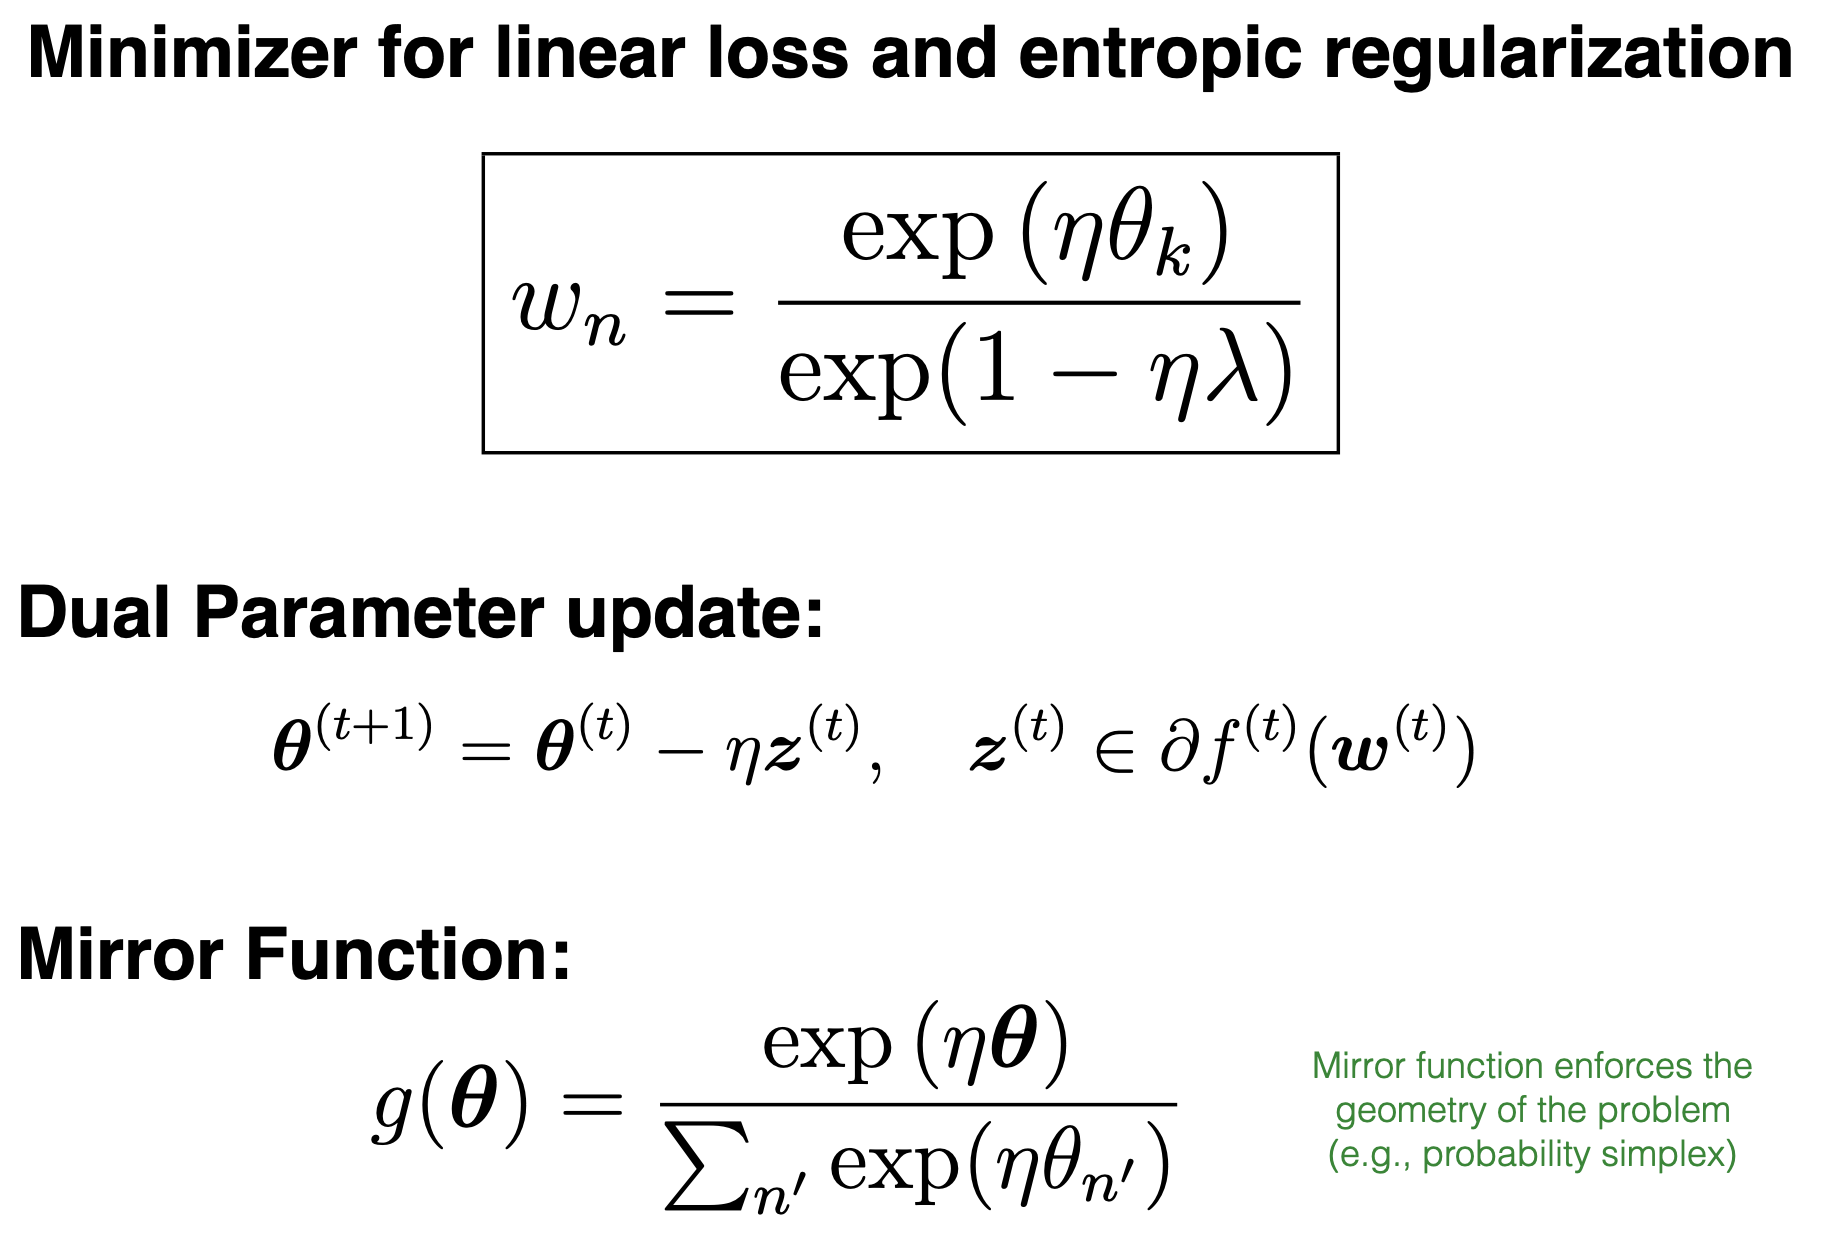
\includegraphics[width=0.6\linewidth]{Img/summary_minimizer_OND.png}
% \end{center}
% \vspace{-10mm}
% %  \caption{Bredman divergence.}
% % \label{fig:breg}
% \end{figure}

Since now we have the rule for dual parameter update and the mirror function, Online Normalized Exponentiated Gradient Descent then can the be arranged in the Algorithm~\ref{algo:onegd2}.

\begin{algorithm}[H]
\caption{Online Norm-Exp-GD ($\eta$)}
\label{algo:onegd2}
\begin{algorithmic}[1]
\FOR{$t=1,\;\cdots,\;T$}
%
\STATE $\btheta^{(t+1)}  = \btheta^{(t)} - \eta \bz^{(t)},  \bz^{(t)} \in \partial f^{(t)}(\bw^{(t)})$ \hfill $\triangleright$ Dual parameter update
%
\STATE $\bw^{(t+1)} \propto \exp{(\eta \btheta^{(t+1)})}$ \hfill $\triangleright$ Mirror projection
%
\ENDFOR
\end{algorithmic}
\end{algorithm}

Let's make the connection to ONEGD more clear as follows:
\begin{align}\label{eq:onegd}
    \bw_n^{(t+1)} = &  \frac{\exp \left(\eta \btheta_n^{(t+1)}\right)}{\sum_{n'} \exp (\eta \btheta_{n'})} \nonumber \\
    = &  \frac{\exp \left(\eta (\btheta_n^{(t)} - \bz_n^{(t)})\right) }{\sum_{k} \exp \left( \eta (\btheta_k^{(t)} - \bz_k^{(t)}) \right)} \nonumber \\
    = & \exp (\eta \btheta_n^{(t)}) \frac{\exp (-\eta \bz_n^{(t)})}{\sum_k \exp (\eta \btheta_k^{(t)}) \exp (-\eta \bz_k^{(t)})} \cdot \frac{\sum_j \exp (\eta \btheta_j^{(t)})}{\sum_j \exp (\eta \btheta_j^{(t)})} \nonumber \\
    = & \frac{\bw_n^{(t)} \exp (-\eta \bz_n^{(t)})}{\sum_k \bw_k^{(t)} \exp (- \eta \bz_k^{(t)})}
\end{align}
%
From equation~\ref{eq:onegd}, we can see it exhibits the same update as the weighted majority algorithm without normalizing:
%
$$ \bw_n^{(t+1)} \propto \bw_n^{(t)} \exp (-\eta \bz_n^{(t)}).$$

Let's review the Hedge algorithm which is presented in Algorithm~\ref{algo:rwma}.
%
\begin{algorithm}[H]
\caption{Hedge algorithm}
\label{algo:rwma}
\begin{algorithmic}[1]
\STATE $\textbf{w}^{(1)} \leftarrow \{\bw_n^{(1)}=1\}_{n=1}^N$ \hfill $\triangleright$ Weight initialization
% \STATE $\eta\leq\frac{1}{2}$\hfill $\triangleright$ Penalty rate initialization
\FOR{$t=1,\;\cdots,\;T$}
\STATE \textsc{Receive} ($\textbf{x}^{(t)}\in\{-1, 1\}^N$) \hfill $\triangleright$ Receive experts predictions
\STATE $I\sim$ \textsc{Multinomial}($\textbf{w}^{(t)}/\Phi^{(t)}$), where $\Phi^{(t)}=\sum_{n=1}^Nw_n^{(t)}$
\STATE $\hat{y}^{(t)}=h_i(\textbf{x}^{(t)})$ \hfill $\triangleright$ Make learner prediction via sampling
\STATE \textsc{Receive} ($y^{(t)}\in\{-1, 1\}$) \hfill $\triangleright$ Receive actual answer
\STATE $\bw_n^{(t+1)} =  \bw_n^{(t)}e^{-\beta\cdot\textbf{1}[y^{(t)}\neq h_n(\textbf{x})^{(t)}]}$ \hfill $\triangleright$ Weight update
% \STATE $w_n^{(t+1)} =  w_n^{(t)}\big(1-\eta\cdot\textbf{1}[y^{(t)}\neq h_n(\textbf{x})^{(t)}]\big)$ \hfill $\triangleright$ Weight update
\ENDFOR
\end{algorithmic}
\end{algorithm}
%
You can see this is actually the unnormalized exponentiated gradient descent, which comes from entropic regularization.
%\section*{References}
%Include your references here. Please cite any resources you found useful.	
%Populate the refs.bib file or list your references manually. Be consistent in formatting!



{
\bibliography{refs}
\bibliographystyle{abbrv}
}

\section{Appendix}
%This section provides any relevant background material that was not covered in the lectures, but was found to be useful for understanding the material. 
%For example, derivations, theory underlying techniques employed, etc. 

%Additionally, this section can summarizes applications or extensions of these techniques found in the literature. 

\subsection{Lipschitz continuity}
\label{sec:l_smooth}

A Lipschitz continuous function $f$ is a function that is limited how fast it can change by a Lipschitz constant $L$~\cite{l_smooth}. The Lipschitz constant $L$ represents the absolute value of the slope of 2 lines. These 2 lines when sliding along the function $f$ itself, would never touch the function $f$ itself. The concept is illustrated in Figure~\ref{fig:l_smooth}.
%
\begin{figure}[h]
    \centering
    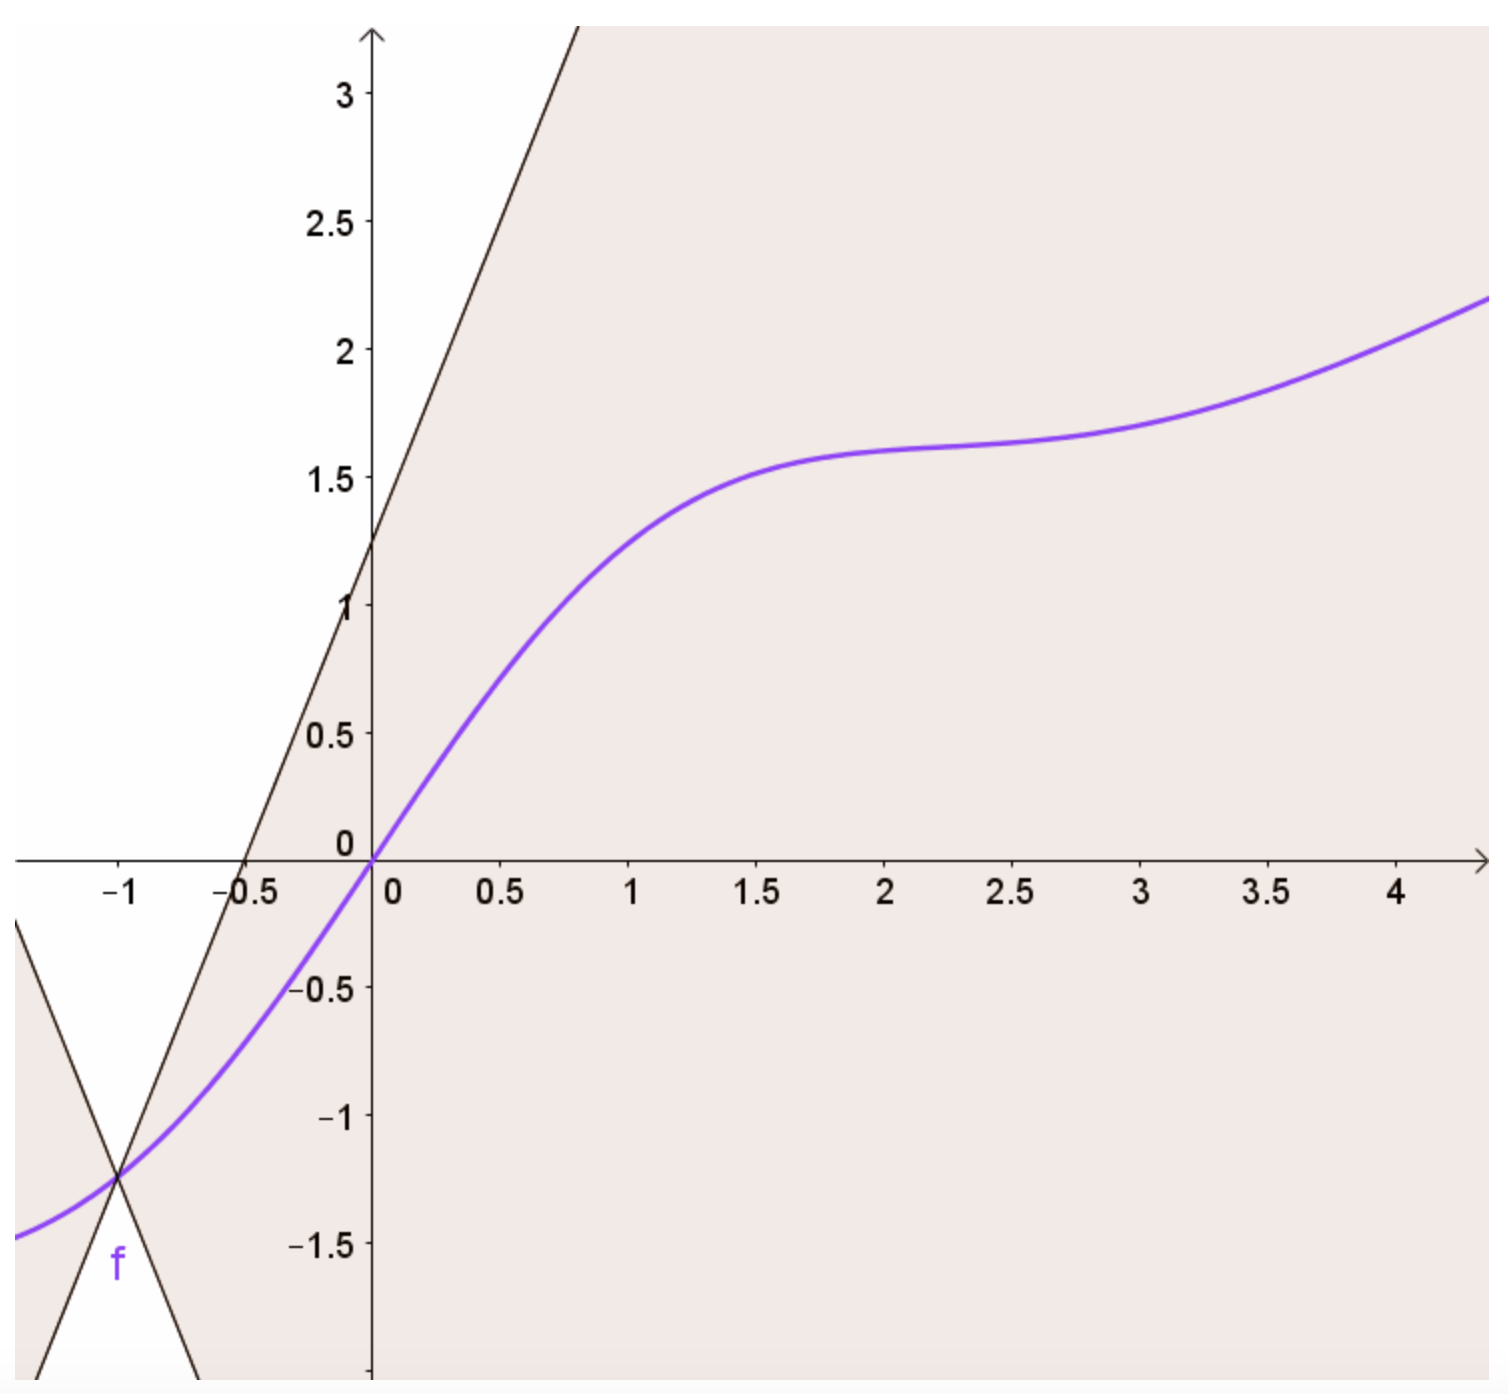
\includegraphics[width=0.6\textwidth]{Img/l_smooth.png}
    \caption{Concept of a Lipschitz continuous function. (Image from Wikipedia~\cite{l_smooth})}
    \label{fig:l_smooth}
\end{figure}
%
Formally, a function $f(\cdot)$ is called a L-Lipschitz continuous function over a set $S$ with respect to a metric $\|\cdot\|$ if for all $\bu, \bw \in S$:
%
\begin{equation*}
\begin{split}
|f(\bu)-f(\bw)| \leq L \|\bu-\bw \|
\end{split}
\end{equation*}
%
With this property, we can proof that the function $f$ is upper bounded by:
%
\begin{equation*}
\begin{split}
f(\bu) \leq f(\bw) + (\bu-\bw)^T \nabla f(\bw) + \frac{L}{2} \|\bu-\bw\|^2_2
\end{split}
\end{equation*}
%
Here, we rephrase the above property as the following lemma~\cite{nonlinear_programming}.

\begin{lemma}[Descent Lemma]
Let $f:\mathbb{R}^n \rightarrow \mathbb{R}$ be continously differentiable, and let $x$ and $y$ be two vectors in $R^n$. Suppose that
\begin{equation*}
\begin{split}
\|\nabla f(x+ty) - \nabla f(x)\| \leq L t\|y\|, \quad \forall t \in [0, 1],
\end{split}
\end{equation*}
where $L$ is some scalar. Then
\begin{equation*}
\begin{split}
f(x+y) \leq f(x) + y'\nabla f(x) + \frac{L}{2} \|y\|^2
\end{split}
\end{equation*}
\end{lemma}

\begin{proof}
Let $t$ be a scalar parameter and let $g(t)=f(x+ty)$. The chain rule yields $(dg/dt)(t) = y'\nabla f(x+ty)$. Now
\begin{equation*}
\begin{split}
f(x+y) - f(x)
&= g(1) - g(0)
= \int_0^1 \frac{dg}{dt}(t)dt = \int_0^1 y' \nabla f(x+ty)dt \\
&\leq \int_0^1 y'\nabla f(x) dt + \Bigg| \int_0^1 y'(\nabla f(x+ty) - \nabla f(x))dt \Bigg| \\
&\leq \int_0^1 y'\nabla f(x) dt +  \int_0^1 \|y\| \cdot \|\nabla f(x+ty) - \nabla f(x)\|dt \\
&\leq y'\nabla f(x) + \|y\| \int_0^1 Lt\|y\|dt \\
&= y'\nabla f(x) + \frac{L}{2} \|y\|^2.
\end{split}
\end{equation*}
\end{proof}

% \textsc{Proof:} 



\end{document} % Done!


